\documentclass[a4paper,12pt]{article}
\usepackage{circuitikz}
\usepackage{graphicx}
\usepackage{amsmath}
\usepackage{amsfonts}
\usepackage{fancyhdr}
\usepackage{geometry}
\usepackage{float}
\geometry{top=1in, bottom=1in, left=1in, right=1in}
\title{Assignment-2\\RC Circuit Response to Square Wave Input}
\author{EE24BTECH11048:NITHIN.K,\\EE24BTECH11021:ESHAN RAY}
\date{\today}
\begin{document}

\maketitle
\section{Function generator}
A \textbf{function generator} is an electronic test equipment used to produce different types of electrical waveforms. These waveforms are typically used for testing circuits, devices, and systems, simulating signals in a controlled environment. Below is an overview of the key features and types of waveforms that a function generator can produce.

\section*{Types of Waveforms}
\begin{itemize}
    \item \textbf{Sine Wave}: A smooth, periodic oscillation. Common in AC power systems and audio applications.
    \item \textbf{Square Wave}: A waveform that alternates between two levels (high and low) with a 50\% duty cycle. Used in digital electronics and clocking circuits.
    \item \textbf{Triangle Wave}: A waveform that linearly rises and falls, used for audio testing and modulation studies.
    \item \textbf{Sawtooth Wave}: A ramp-up waveform followed by a sudden drop, often used in TV signal generation and audio applications.
    \item \textbf{Pulse Wave}: Similar to a square wave but with adjustable duty cycles (the proportion of time the signal stays high). It’s used in time-based measurements.
    \item \textbf{Arbitrary Waveform}: Allows the creation of custom waveforms, typically via a digital interface, to replicate specific signal patterns for more specialized testing.
\end{itemize}

\section*{Key Parameters}
\begin{itemize}
    \item \textbf{Frequency}: The number of cycles per second (Hz). Most function generators can cover a wide frequency range, from low-frequency (e.g., 1 Hz) to high-frequency (e.g., several MHz or even GHz).
    \item \textbf{Amplitude}: The peak value of the signal, usually adjustable.
    \item \textbf{Offset}: The vertical shift of the waveform, allowing the signal to be centered at a desired voltage.
    \item \textbf{Duty Cycle}: The fraction of the period in which the signal is high (for square and pulse waves).
    \item \textbf{Waveform Symmetry}: Controls how the waveform behaves symmetrically or asymmetrically.
\end{itemize}

\section*{Features}
\begin{itemize}
    \item \textbf{Adjustable Frequency}: Most function generators allow fine control over frequency, from micro-hertz to gigahertz ranges.
    \item \textbf{Amplitude Control}: The signal's peak-to-peak voltage can be adjusted to meet the needs of a specific test circuit.
    \item \textbf{Waveform Selection}: Users can select different waveform shapes (sine, square, triangle, etc.) depending on the requirements of their test.
    \item \textbf{Modulation}: Some function generators can modulate the output signal, which is useful for simulating AM, FM, or PM signals.
    \item \textbf{Digital Interface}: Higher-end function generators may come with the ability to connect to a computer for remote control or signal analysis.
\end{itemize}

\section*{Applications}
\begin{itemize}
    \item \textbf{Testing Circuits}: Commonly used for testing amplifiers, oscillators, and other signal processing devices.
    \item \textbf{Simulation}: Simulating real-world signals such as communication signals, audio signals, or video signals for troubleshooting and development.
    \item \textbf{Signal Processing}: Used in signal processing and control systems to generate reference signals for various systems.
\end{itemize}

\section*{Types of Function Generators}
\begin{itemize}
    \item \textbf{Analog Function Generators}: Older type that directly generates sine waves and other basic waveforms through analog circuitry. They can suffer from limitations in waveform quality and frequency stability.
    \item \textbf{Digital (Arbitrary) Function Generators}: These are more advanced and allow users to define complex waveforms with higher precision. They often use digital-to-analog converters (DACs) to output the signal, offering greater flexibility in terms of waveform types and accuracy.
\end{itemize}



\section{Introduction to RC Circuits}
RC circuits (Resistor-Capacitor circuits) are widely used in various applications across electronics and engineering. Some common uses include:

\subsection{1. Signal Processing}
\begin{itemize}
    \item \textbf{Filters (Low-pass, High-pass, Band-pass, Band-stop)}: Used in audio processing, communication systems, and signal conditioning.
    \item \textbf{Integrators and Differentiators}: Used in analog computers and signal shaping.
\end{itemize}

\subsection{2. Timing and Oscillators}
\begin{itemize}
    \item \textbf{Timers (e.g., 555 Timer Circuits)}: Used in pulse generation, LED blinking, and clock circuits.
    \item \textbf{Oscillators (e.g., RC phase shift oscillator)}: Used in waveform generators and audio circuits.
\end{itemize}

\subsection{3. Power Supply Circuits}
\begin{itemize}
    \item \textbf{Smoothing Circuits}: In power supplies, capacitors smooth out voltage fluctuations after rectification.
    \item \textbf{Snubber Circuits}: Used to protect switches (e.g., relays and transistors) from voltage spikes.
\end{itemize}

\subsection{4. Communication Systems}
\begin{itemize}
    \item \textbf{Coupling and Decoupling Capacitors}: Block DC and allow AC signals in amplifier and radio circuits.
    \item \textbf{Tuned Circuits}: Used in radio receivers for frequency selection.
\end{itemize}

\subsection{5. Medical and Biomedical Applications}
\begin{itemize}
    \item \textbf{ECG Signal Processing}: Used to filter noise in electrocardiogram (ECG) circuits.
    \item \textbf{Defibrillators}: Store and release charge to restore heart rhythm.
\end{itemize}

\subsection{6. Sensor and Measurement Systems}
\begin{itemize}
    \item \textbf{Capacitive Touch Sensors}: Used in touchscreens and proximity sensors.
    \item \textbf{RC Time Constant Measurement}: Helps in capacitance and resistance measurement.
\end{itemize}

\begin{figure}[H]
    \centering
    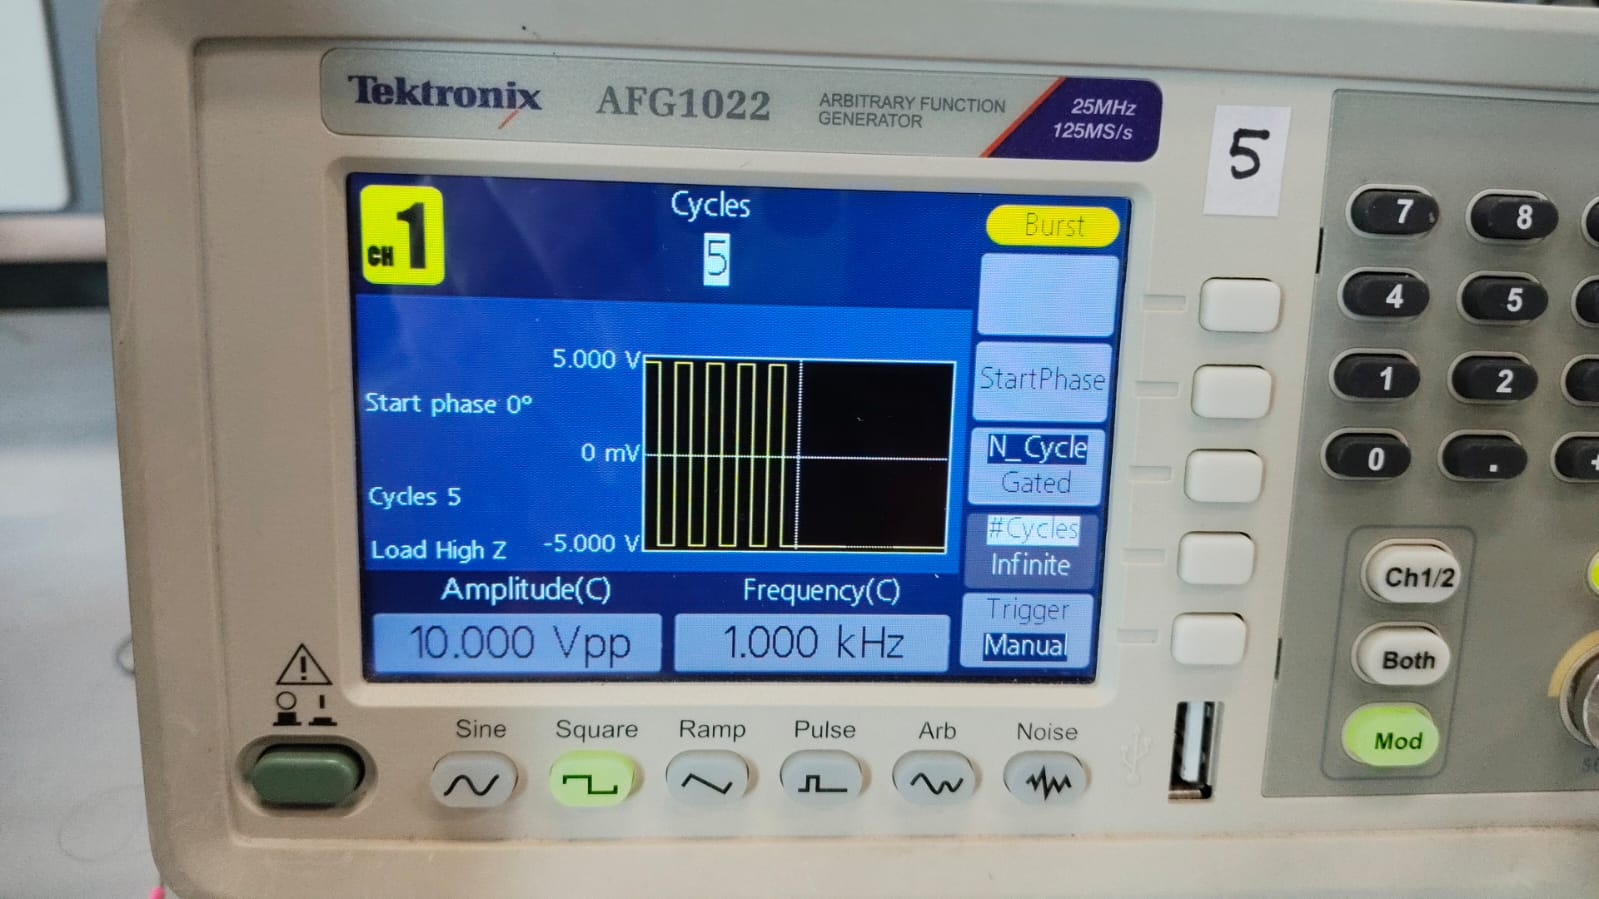
\includegraphics[width=\textwidth]{figs/func_gen.jpeg}
\end{figure}

\section{RC Filters}

\subsection{1. Low-Pass Filter}
\begin{center}
\begin{circuitikz}
    \draw (0,0) to [R, l=$R$] (2,0) to [C, l=$C$] (2,-2) -- (0,-2) -- (0,0);
    \draw (2,0) -- (3,0);
    \node at (3.5,0) {Vout};
    \node at (-0.5,0) {Vin};
    \node at (1,-2.5) {GND};
\end{circuitikz}
\end{center}

\textbf{Explanation:}
\begin{itemize}
    \item \textbf{Vin (Input Voltage)}: The signal applied to the circuit.
    \item \textbf{R (Resistor)}: Controls the rate at which the capacitor charges and discharges.
    \item \textbf{C (Capacitor)}: Stores and releases charge, filtering high-frequency signals.
    \item \textbf{Vout (Output Voltage)}: The filtered signal is taken across the capacitor.
    \item \textbf{GND (Ground)}: Reference potential for the circuit.
\end{itemize}

\textbf{Functioning:}
\begin{itemize}
    \item \textbf{Low Frequencies}: The capacitor has high impedance, so most of the input voltage appears across it, allowing low frequencies to pass.
    \item \textbf{High Frequencies}: The capacitor's impedance decreases, shorting high-frequency signals to ground, effectively filtering them out.
\end{itemize}

\textbf{Cutoff Frequency:} 
The cutoff frequency \( f_c \) is given by:
\[
    f_c = \frac{1}{2\pi RC}
\]
Frequencies below \( f_c \) pass with minimal attenuation, while frequencies above \( f_c \) are progressively attenuated.

\subsection{2. High-Pass Filter}
\begin{center}
\begin{circuitikz}
    \draw (0,0) to [C, l=$C$] (2,0) to [R, l=$R$] (2,-2) -- (0,-2) -- (0,0);
    \draw (2,0) -- (3,0);
    \node at (3.5,0) {Vout};
    \node at (-0.5,0) {Vin};
    \node at (1,-2.5) {GND};
\end{circuitikz}
\end{center}

\textbf{Explanation:}
\begin{itemize}
    \item \textbf{Vin (Input Voltage)}: The applied signal.
    \item \textbf{C (Capacitor)}: Blocks low-frequency signals but allows high frequencies to pass.
    \item \textbf{R (Resistor)}: Forms a voltage divider with the capacitor.
    \item \textbf{Vout (Output Voltage)}: The filtered signal is taken across the resistor.
    \item \textbf{GND (Ground)}: Reference potential for the circuit.
\end{itemize}

\textbf{Functioning:}
\begin{itemize}
    \item \textbf{High Frequencies}: The capacitor has low impedance, allowing high-frequency signals to pass to the output.
    \item \textbf{Low Frequencies}: The capacitor has high impedance, blocking low-frequency signals and attenuating them.
\end{itemize}

\textbf{Cutoff Frequency:} 
The cutoff frequency \( f_c \) is given by:
\[
    f_c = \frac{1}{2\pi RC}
\]
Frequencies above \( f_c \) pass with minimal attenuation, while frequencies below \( f_c \) are progressively attenuated.

\subsection{3. Band-Pass Filter}
\begin{center}
\begin{circuitikz}
    \draw (0,0) to [C, l=$C_1$] (2,0) to [R, l=$R$] (2,2) to [C, l=$C_2$] (4,2) -- (4,0) -- (6,0);
    \node at (6.5,0) {Vout};
    \node at (-0.5,0) {Vin};
    \node at (3,-2.5) {GND};
\end{circuitikz}
\end{center}

\textbf{Explanation:}
\begin{itemize}
    \item \textbf{C1 (High-Pass Section)}: Blocks low frequencies and passes higher ones.
    \item \textbf{R1 (High-Pass Resistor)}: Forms an RC circuit with C1, setting the lower cutoff frequency \( f_L \).
    \item \textbf{R2 (Low-Pass Resistor)}: Works with C2 (if present) to filter out high frequencies, setting the upper cutoff frequency \( f_H \).
\end{itemize}

\textbf{Functioning:}
\begin{itemize}
    \item Frequencies below \( f_L \) are attenuated by the HPF section.
    \item Frequencies above \( f_H \) are attenuated by the LPF section.
    \item Frequencies between \( f_L \) and \( f_H \) pass through with minimal attenuation.
\end{itemize}

\textbf{Cutoff Frequencies:}
The lower cutoff frequency \( f_L \) is set by the high-pass filter:
\[
    f_L = \frac{1}{2\pi R_1 C_1}
\]
The upper cutoff frequency \( f_H \) is set by the low-pass filter:
\[
    f_H = \frac{1}{2\pi R_2 C_2}
\]
The bandwidth of the filter is:
\[
    \text{Bandwidth} = f_H - f_L
\]

\subsection{4. Band-Stop Filter}
\begin{center}
\begin{circuitikz}
    \draw (0,0) to [R, l=$R$] (2,0) to [C, l=$C_1$] (2,2) -- (4,2) to [R, l=$R$] (4,0) to [C, l=$C_2$] (6,0);
    \node at (6.5,0) {Vout};
    \node at (-0.5,0) {Vin};
    \node at (3,-2.5) {GND};
\end{circuitikz}
\end{center}

\textbf{Explanation:}
\begin{itemize}
    \item \textbf{R1 \& C1 (Low-Pass Section)}: Blocks high frequencies and passes lower ones.
    \item \textbf{R2 \& C2 (High-Pass Section)}: Blocks low frequencies and passes higher ones.
    \item \textbf{Parallel Configuration}: Frequencies in the stop band are attenuated, while others pass.
\end{itemize}

\textbf{Functioning:}
\begin{itemize}
    \item Frequencies below \( f_L \) pass through the low-pass section.
    \item Frequencies above \( f_H \) pass through the high-pass section.
    \item Frequencies between \( f_L \) and \( f_H \) are attenuated, forming a notch in the response.
\end{itemize}

\textbf{Cutoff Frequencies:}
The lower cutoff frequency \( f_L \) is set by the low-pass filter:
\[
    f_L = \frac{1}{2\pi R_1 C_1}
\]
The upper cutoff frequency \( f_H \) is set by the high-pass filter:
\[
    f_H = \frac{1}{2\pi R_2 C_2}
\]
The notch width (stop band) is:
\[
    \text{Notch Width} = f_H - f_L
\]

\subsection{Cutoff Frequency}
For Low-Pass and High-Pass filters:
\begin{equation}
    f_c = \frac{1}{2\pi RC}
\end{equation}

For Band-Pass and Band-Stop filters:
\begin{equation}
    f_c = \frac{1}{2\pi \sqrt{R_1 R_2 C_1 C_2}}
\end{equation}

\section*{Introduction}
In this report, we analyze the response of an RC circuit to a square wave input of $\pm 5V$. The circuit will be analyzed for three different conditions of the time constant \( \tau = RC \) relative to the period \( T \) of the input square wave:

\begin{itemize}
    \item \( RC = T \)
    \item \( RC \gg T \)
    \item \( RC \ll T \)
\end{itemize}

The purpose of this analysis is to observe the transient response for the first five cycles and the steady-state response in each case. The results will be compared with hand calculations and CRO measurements for accuracy.

\section*{Theory}
The general behavior of an RC circuit can be described by the following first-order differential equation for a charging or discharging capacitor:

\[
V_C(t) = V_{max} \left(1 - e^{-\frac{t}{RC}}\right)
\]
where \( V_C(t) \) is the voltage across the capacitor at time \( t \), \( V_{max} \) is the maximum voltage (input voltage), and \( RC \) is the time constant of the circuit.

For a square wave input, the capacitor will charge and discharge between the high and low voltage levels, and the behavior of the output will depend on the relationship between \( RC \) and \( T \).

\section*{Experimental Setup}
The RC circuit is configured with the following components:
\begin{itemize}
    \item Resistor \( R \)
    \item Capacitor \( C \)
    \item Square wave generator providing a \( \pm 5V \) input
    \item Oscilloscope (CRO) to measure the input and output waveforms
\end{itemize}

The measurements were made for each case where the time constant \( RC \) was varied to match the conditions described earlier. The CRO was used to observe the transient and steady-state responses.\\
\section{Procedure:}
Connect the resistor and the capacitor in series and then the probe to the intersection of capacitor and resistor. The ground of the probe and the input ground should be connected to capacitor end and the input should be given to the other end of resistor. The circuit diagram is given below.
\begin{figure}[H]
    \centering
    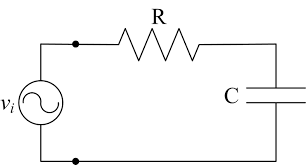
\includegraphics[width=0.5\textwidth]{figs/diagram_cir.png}
\end{figure}

\begin{figure}[H]
    \centering
    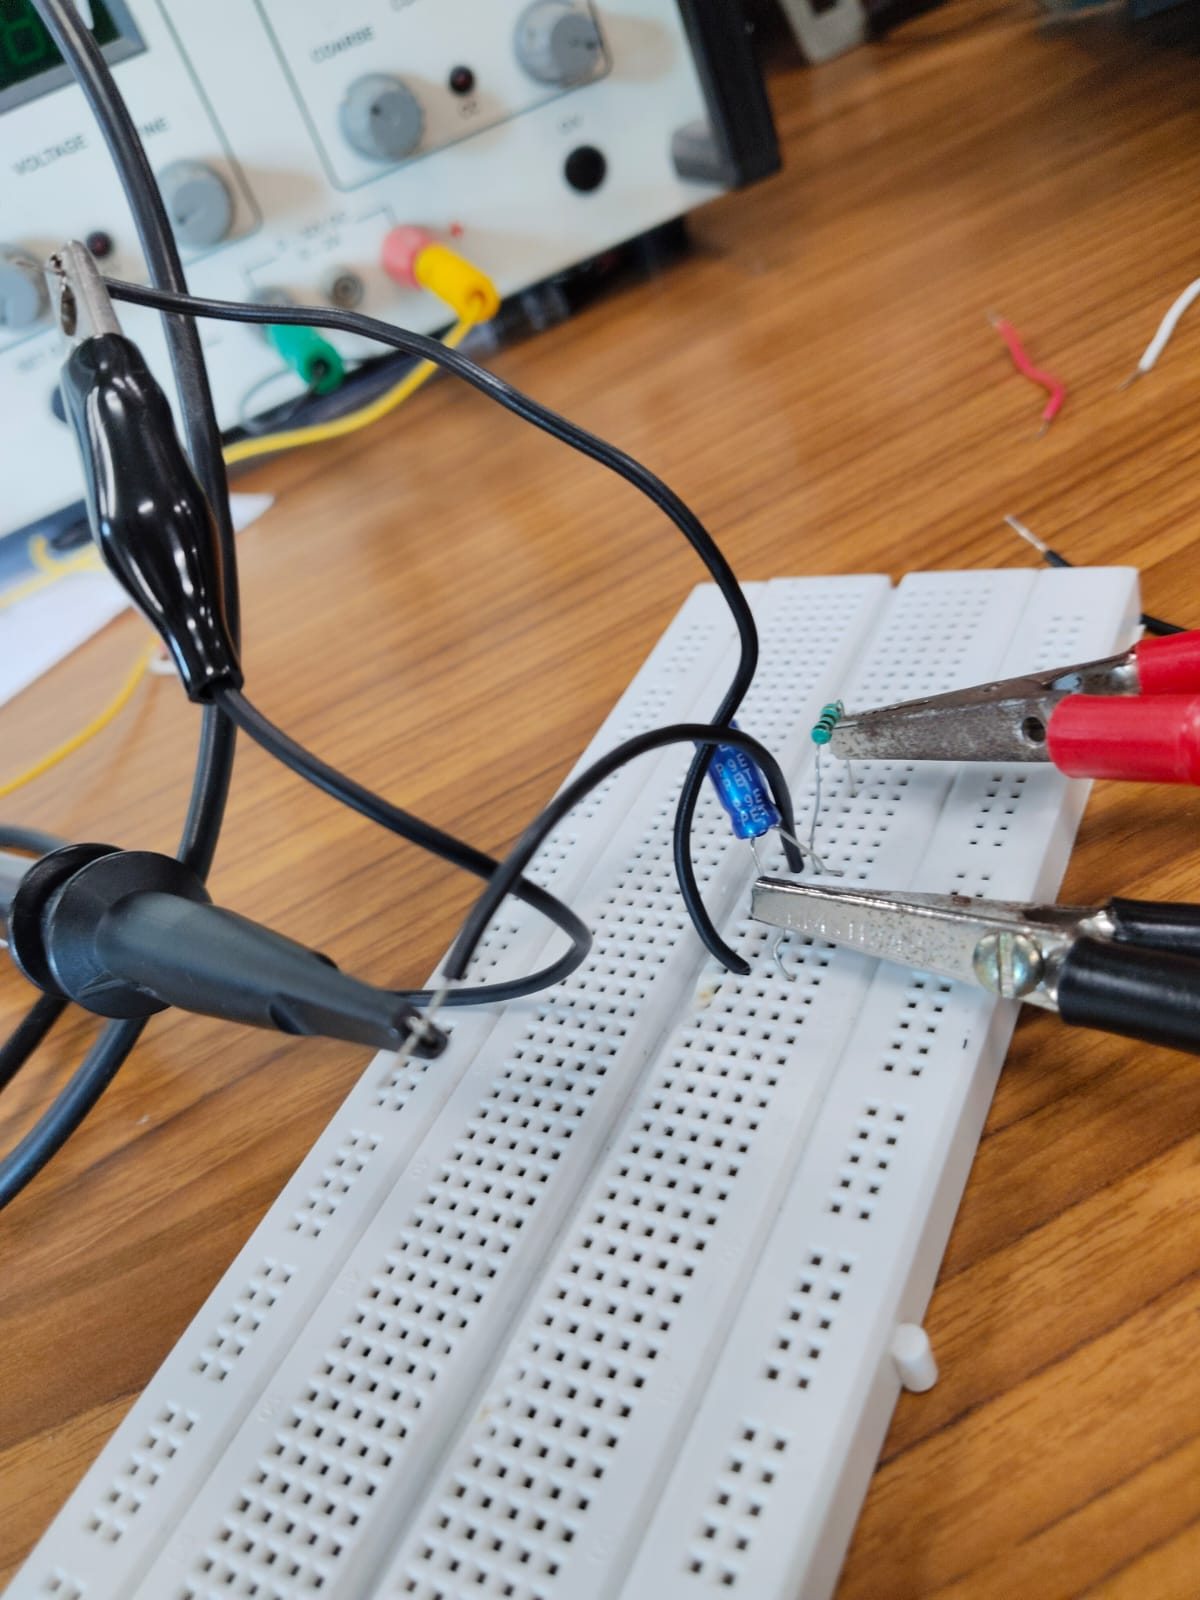
\includegraphics[width=0.5\textwidth]{figs/circuit.jpeg}
    \caption{Circuit}
\end{figure}

\section*{Analysis of the Cases}
\subsection*{Case 1: \( RC = T \)}
When the time constant \( RC \) is equal to the period \( T \) of the square wave, the capacitor charges and discharges over the course of each cycle. The output voltage will follow the input waveform but with some delay and smoothing due to the capacitor charging and discharging.

\[
V_C(t) = V_{max} \left( 1 - e^{-\frac{t}{RC}} \right)
\]
For Calculating Time period :\\
Taking the difference of x-values in the figures below we get T = 300ms - (-680ms) = 980ms
\begin{figure}[H]
    \centering
    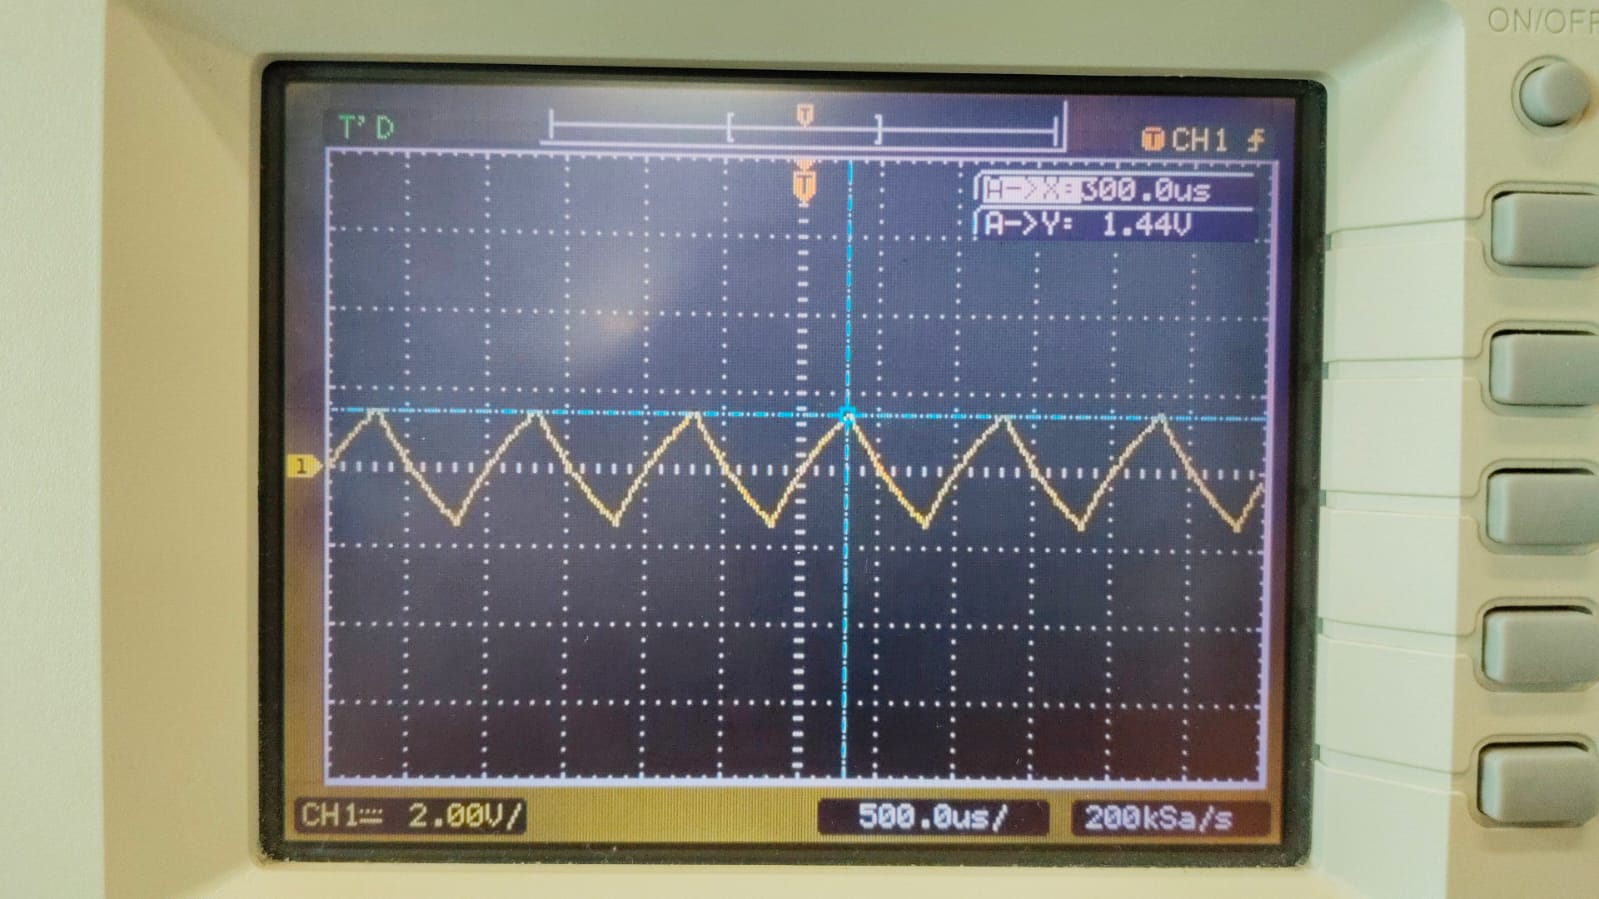
\includegraphics[width=\textwidth]{figs/rc=t_Time.jpeg}
\end{figure}

\subsubsection*{Steady-State Response}
In the steady state, the output voltage will closely match the input waveform but with a delay due to the time required for the capacitor to charge and discharge.

\begin{figure}[H]
    \centering
    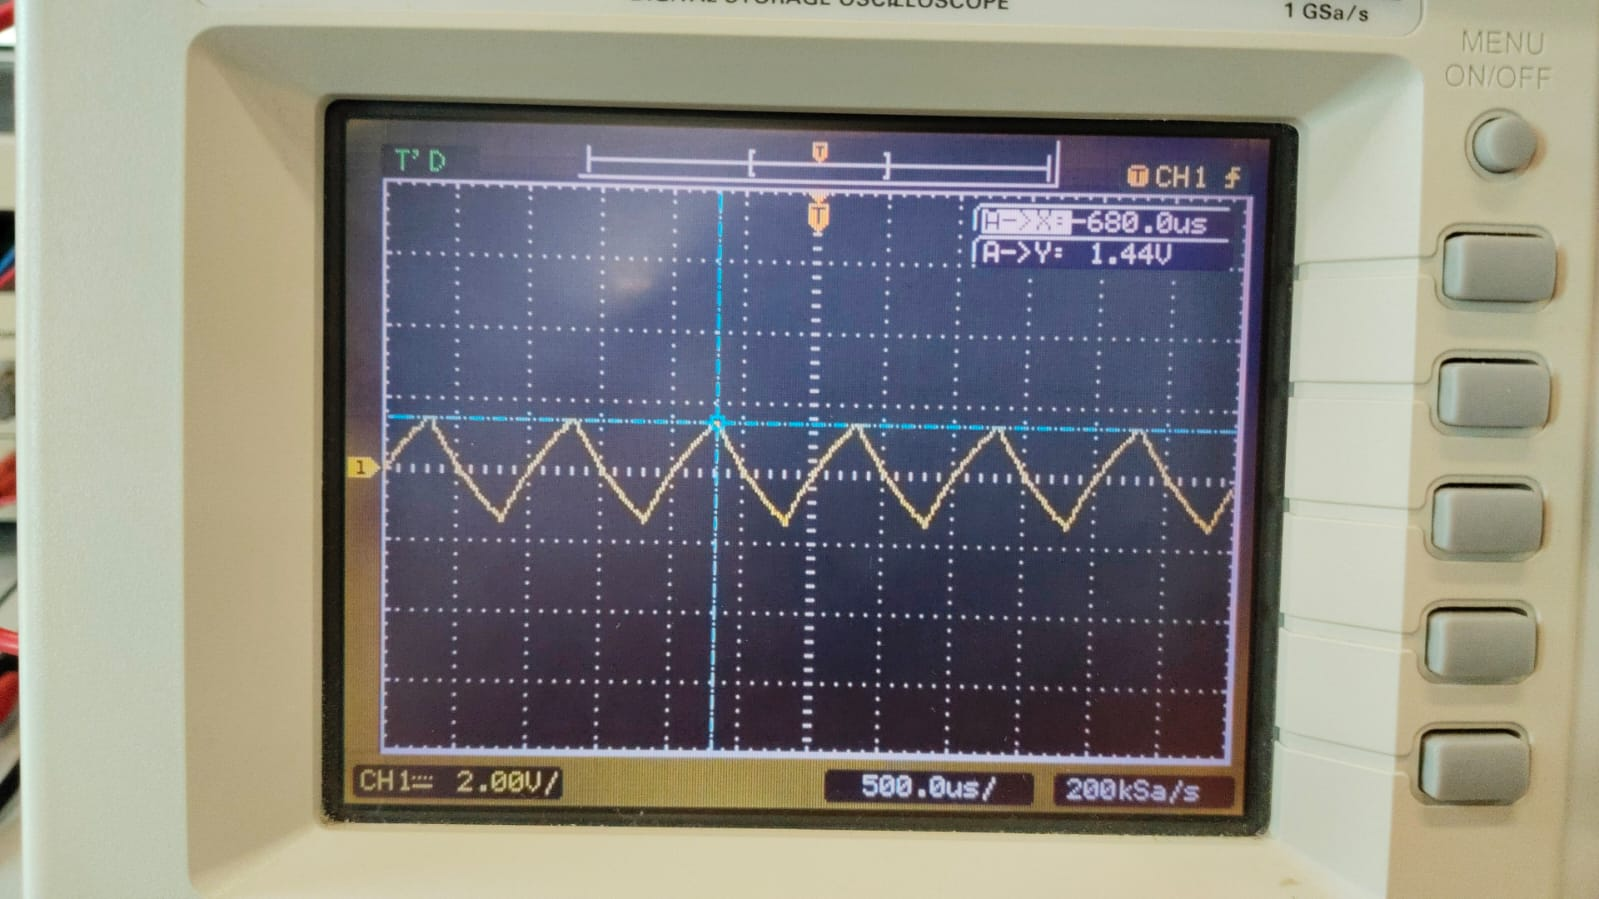
\includegraphics[width=\textwidth]{figs/rc=t.jpeg}
    \caption{Steady-State Response : \( RC = T \)}
\end{figure}
\begin{figure}[H]
    \centering
    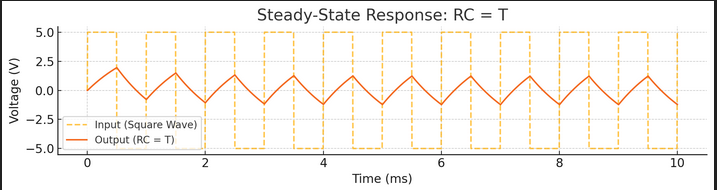
\includegraphics[width=\textwidth]{figs/rc=t_prog.png}
\end{figure}

\subsubsection*{Transient Response Calculation}
For \( RC = T \), the capacitor charges and discharges during each cycle. Let's assume that the input square wave has a period \( T \) and a peak voltage of \( V_{max} = 5V \).

At the start of the cycle, the capacitor is initially uncharged, and the voltage across the capacitor increases according to the equation above. The time constant \( \tau = RC = T \) is the time it takes for the voltage to reach approximately \( 63\% \) of the input value.

To calculate the voltage across the capacitor at any time \( t \), we can use:

\[
V_C(t) = V_{max} \left(1 - e^{-\frac{t}{T}}\right)
\]
Theoretically :
\[
V_C\left(t\right) = 5V \left( 1 - e^{-0.3} \right) \approx 5V \times (1 - 0.74) \approx 5V \times 0.26 \approx 1.3V
\]

Calculation For our experiment, at \( t = 0.3ms \) :

\[
V_C\left(t\right) = 5V \left( 1 - e^{-0.3/0.98} \right) \approx 5V \times (1 - 0.7362) \approx 5V \times 0.2637 \approx 1.32V
\]

Observation(figure 3) :\\the values of the capacitance and resistance were not exact when it was checked with the multimeter hence we got 1.44V\\
\[
\text{Our resistor was } \approx 1.06K\Omega \text{ and the capacitor was } \approx 0.924\mu F \text{ hence } RC = 0.979ms
\]

\begin{figure}[H]
    \centering
    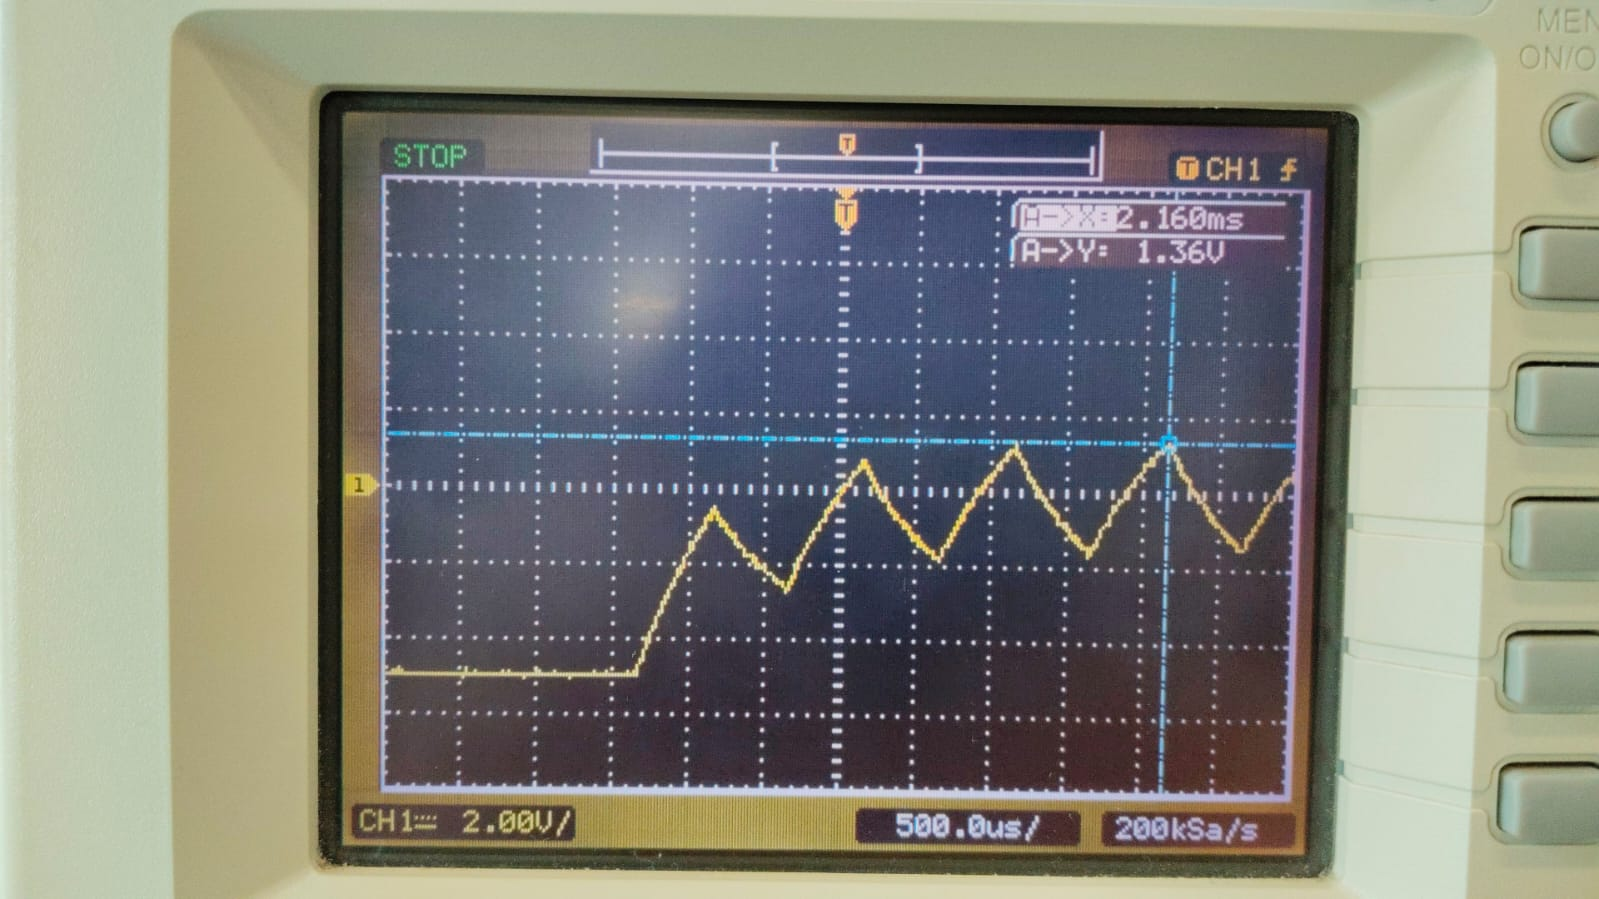
\includegraphics[width=\textwidth]{figs/rc=t_tr.jpeg}
    \caption{Transient Response for the first 5 cycles: \( RC = T \) }
\end{figure}

\subsection*{Case 2: \( RC \gg T \)}
When \( RC \) is much greater than the period \( T \) of the square wave, the capacitor has much more time to charge and discharge, and the output voltage will appear more like a low-pass filter response.

\subsubsection*{Steady-State Response}
In the steady state, the output will closely resemble a smoothed version of the input waveform, with minimal ripple.
\begin{figure}[H]
   \centering
   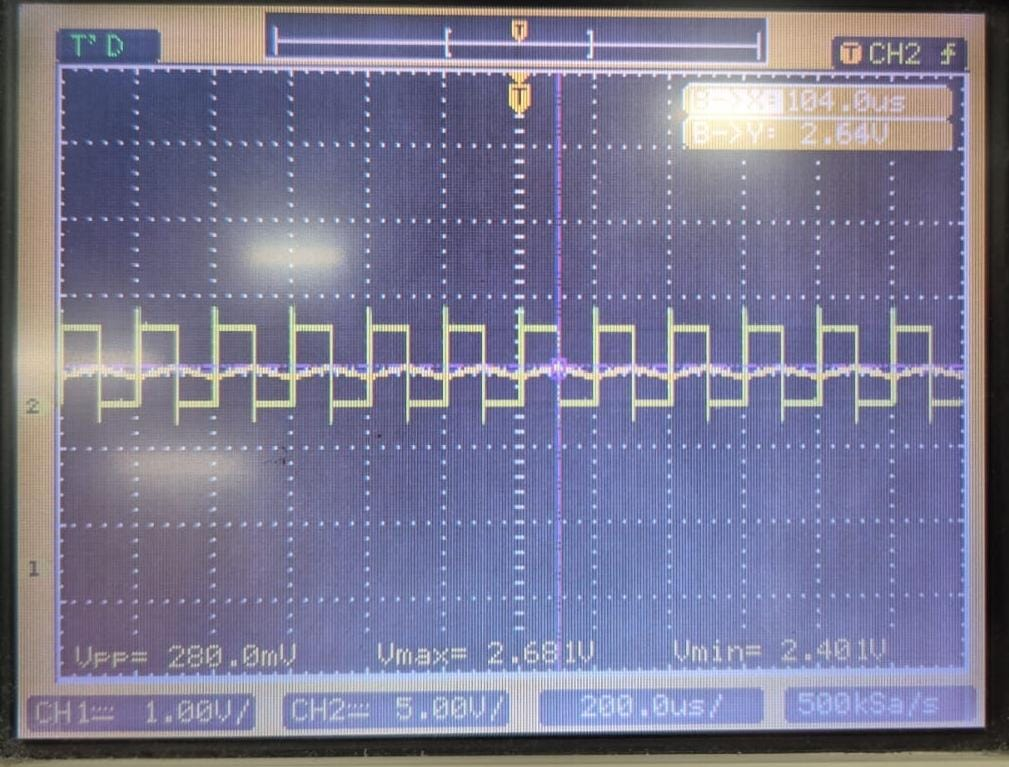
\includegraphics[width=0.8\textwidth]{figs/rc>t.jpeg}
   \caption{Steady-State Response : \( RC \gg T \)}
\end{figure}

\begin{figure}[H]
    \centering
    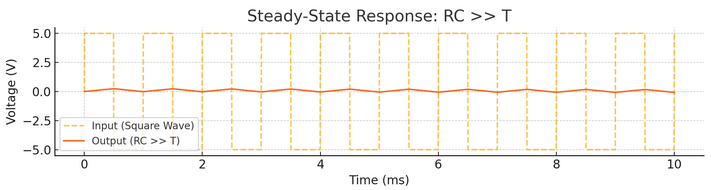
\includegraphics[width=\textwidth]{figs/rc>t_prog.png}
\end{figure}

\subsubsection*{Transient Response Calculation}
For \( RC \gg T \), the capacitor will charge slowly, and the voltage across the capacitor will not reach its final value within one period of the square wave. We can use the equation for capacitor charging:

\[
V_C(t) = V_{max} \left( 1 - e^{-\frac{t}{RC}} \right)
\]

For this case, the capacitor will charge very slowly, and by the time the input square wave changes polarity, the capacitor will have only partially charged.\\

For this case, \( RC = 0.2ms \), T = 0.02ms then after the period \( t = 0.104ms \):\\
theoretically :
\[
V_C\left(t\right) = 5V \left( 1 - e^{-0.104/0.2} \right) \approx 5V \times (1 - 0.59) \approx 5V \times 0.41 \approx 2.05V
\]

The capacitor barely charges before the input reverses polarity.\\

Observation(figure 4) : \\
\[
V_C(t) = 2.64V
\]
Due to some errors in resistor and capacitor values we are getting errors in the voltage. 
\begin{figure}[H]
    \centering
    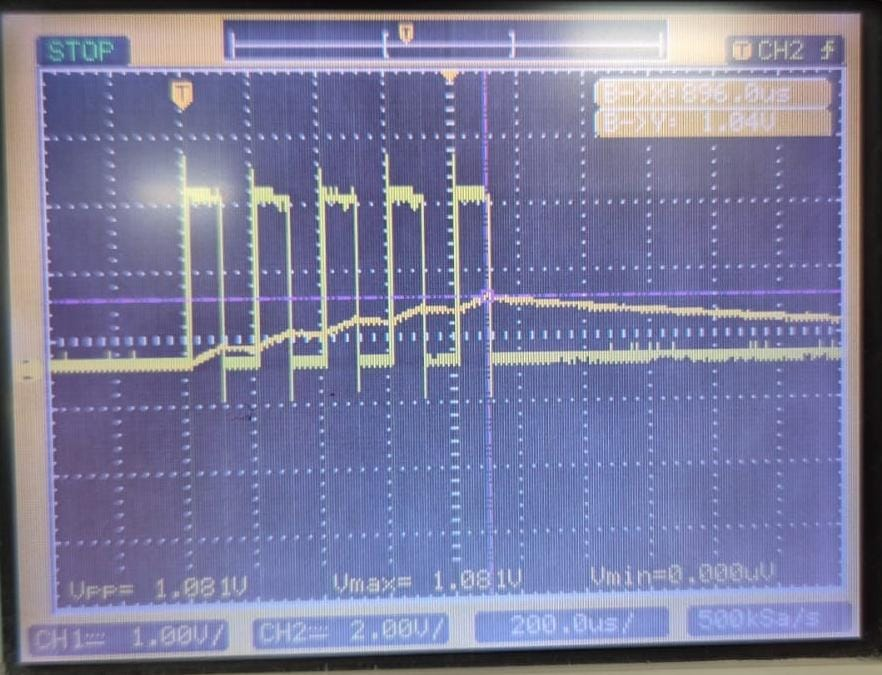
\includegraphics[width=0.8\textwidth]{figs/rc>t_tr.jpeg}
    \caption{Transient Response for the first 5 cycles : \( RC \gg T \)}
\end{figure}

\subsection*{Case 3: \( RC \ll T \)}
When \( RC \) is much smaller than the period \( T \), the capacitor charges and discharges very quickly, and the output voltage will closely follow the input waveform.\\
For Calculating Time period :\\
Taking the difference of x-values in the figures below we get T = 14.2ms - 4.4ms = 9.8ms while the input given was T = 10ms.
\begin{figure}[H]
    \centering
    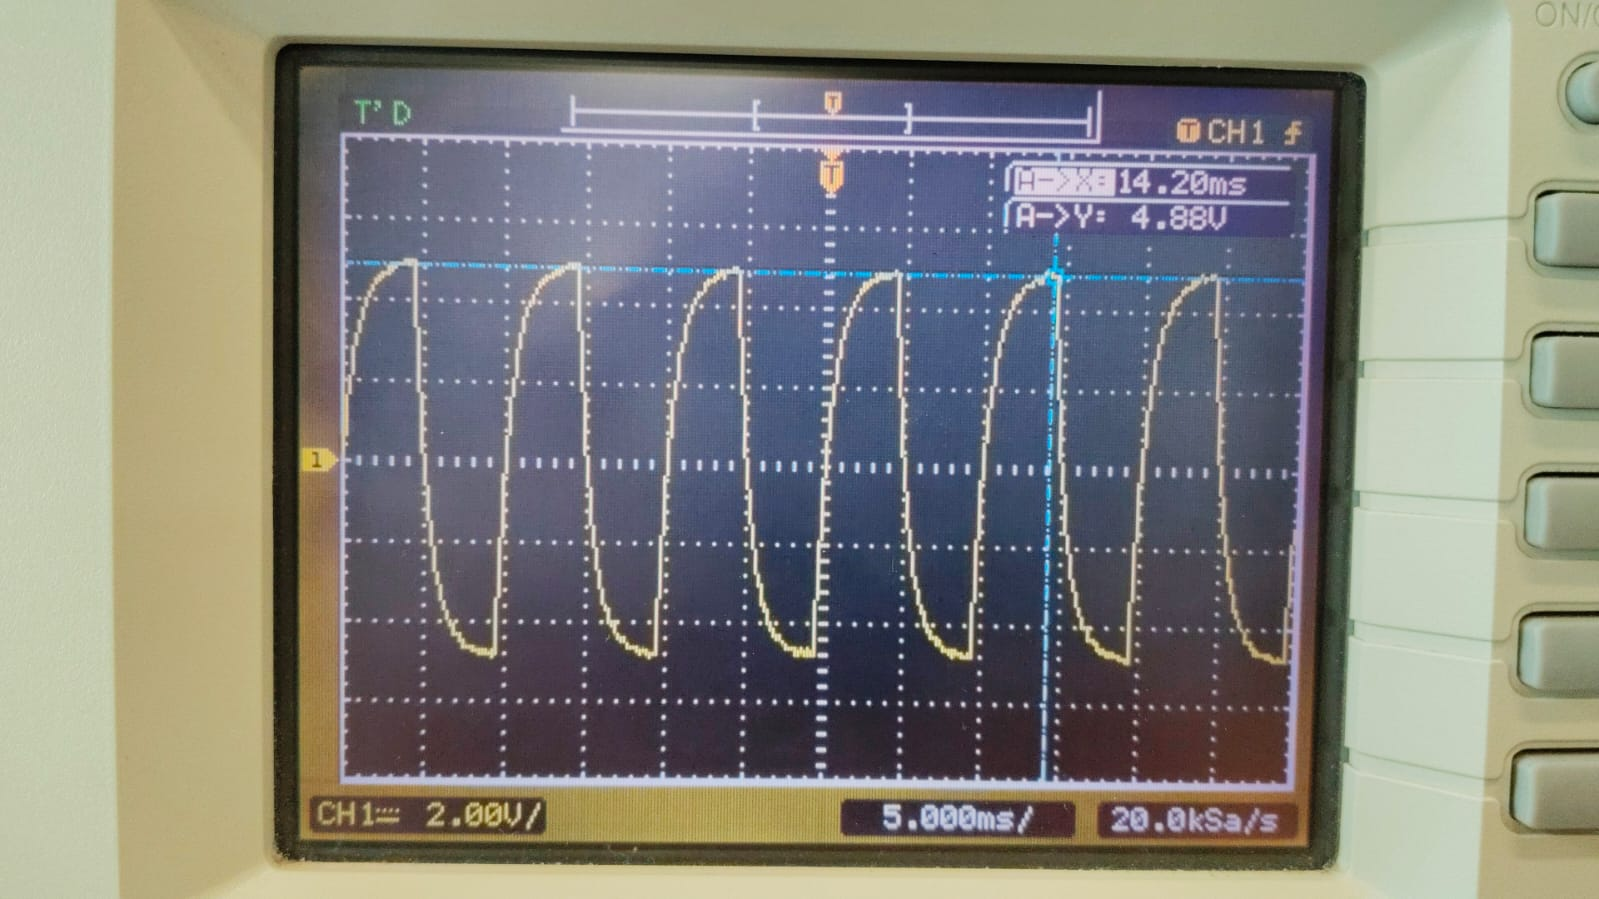
\includegraphics[width=\textwidth]{figs/rc<t_Time.jpeg}
\end{figure}
\subsubsection*{Steady-State Response}
In the steady state, the output voltage will almost exactly match the input waveform with little to no distortion.
\begin{figure}[H]
    \centering
    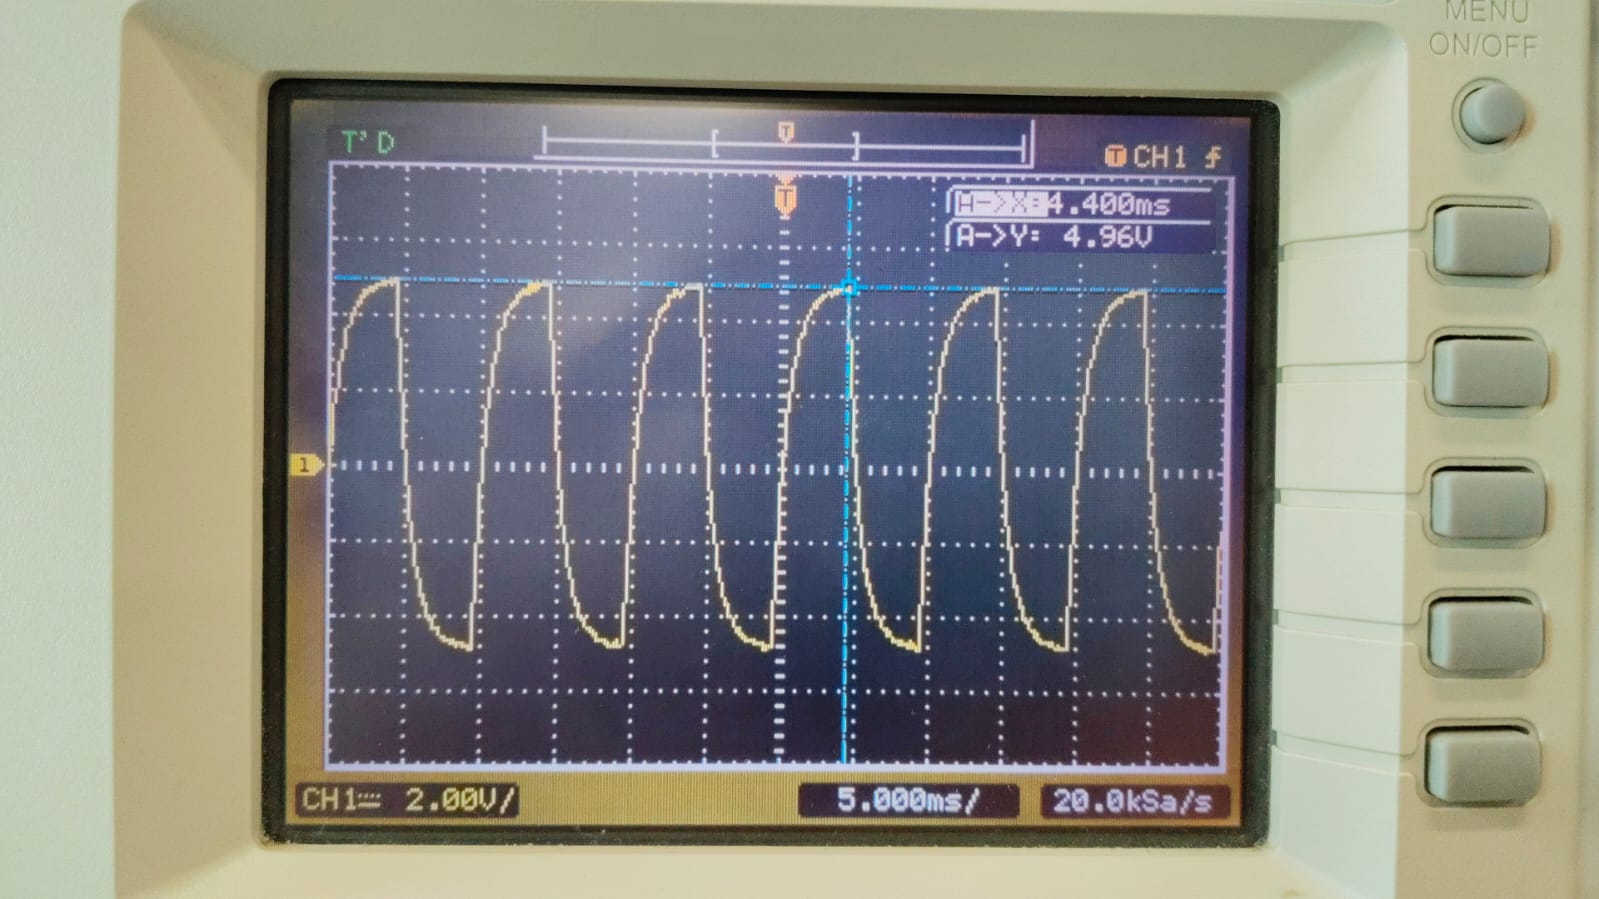
\includegraphics[width=\textwidth]{figs/rc<t.jpeg}
    \caption{Steady-State Response : \( RC \ll T \)}
\end{figure}
\begin{figure}[H]
    \centering
    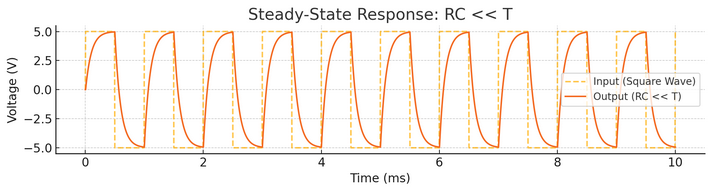
\includegraphics[width=\textwidth]{figs/rc<t_prog.png}
\end{figure}

\subsubsection*{Transient Response Calculation}
For \( RC \ll T \), the capacitor charges and discharges rapidly, and the voltage across the capacitor will track the input waveform closely.

In this case, the capacitor charges almost instantaneously and the output will closely follow the square wave.

For this case theoretically, \( RC = 1ms \), then after a very short time, the voltage across the capacitor will approach \( V_{max} \). 

\[
V_C\left(t\right) \approx V_{max} = 5V
\]

Since the time constant is much smaller than the period of the square wave, the voltage change happens almost instantaneously.

Theoretically :

\[
V_C\left(t\right) = 5V \left( 1 - e^{-4.4} \right) \approx 5V \times (1 - 0.0123) \approx 5V \times 0.9877 \approx 4.9385V
\]

Calculation For our experiment, at \( t = 4.4ms \) :

\[
V_C\left(t\right) = 5V \left( 1 - e^{-4.4/0.98} \right) \approx 5V \times (1 - 0.01123) \approx 5V \times 0.9887 \approx 4.944V
\]

Observation in steady state :
\[
V_C\left(t\right) = 4.96V
\]

\begin{figure}[H]
    \centering
    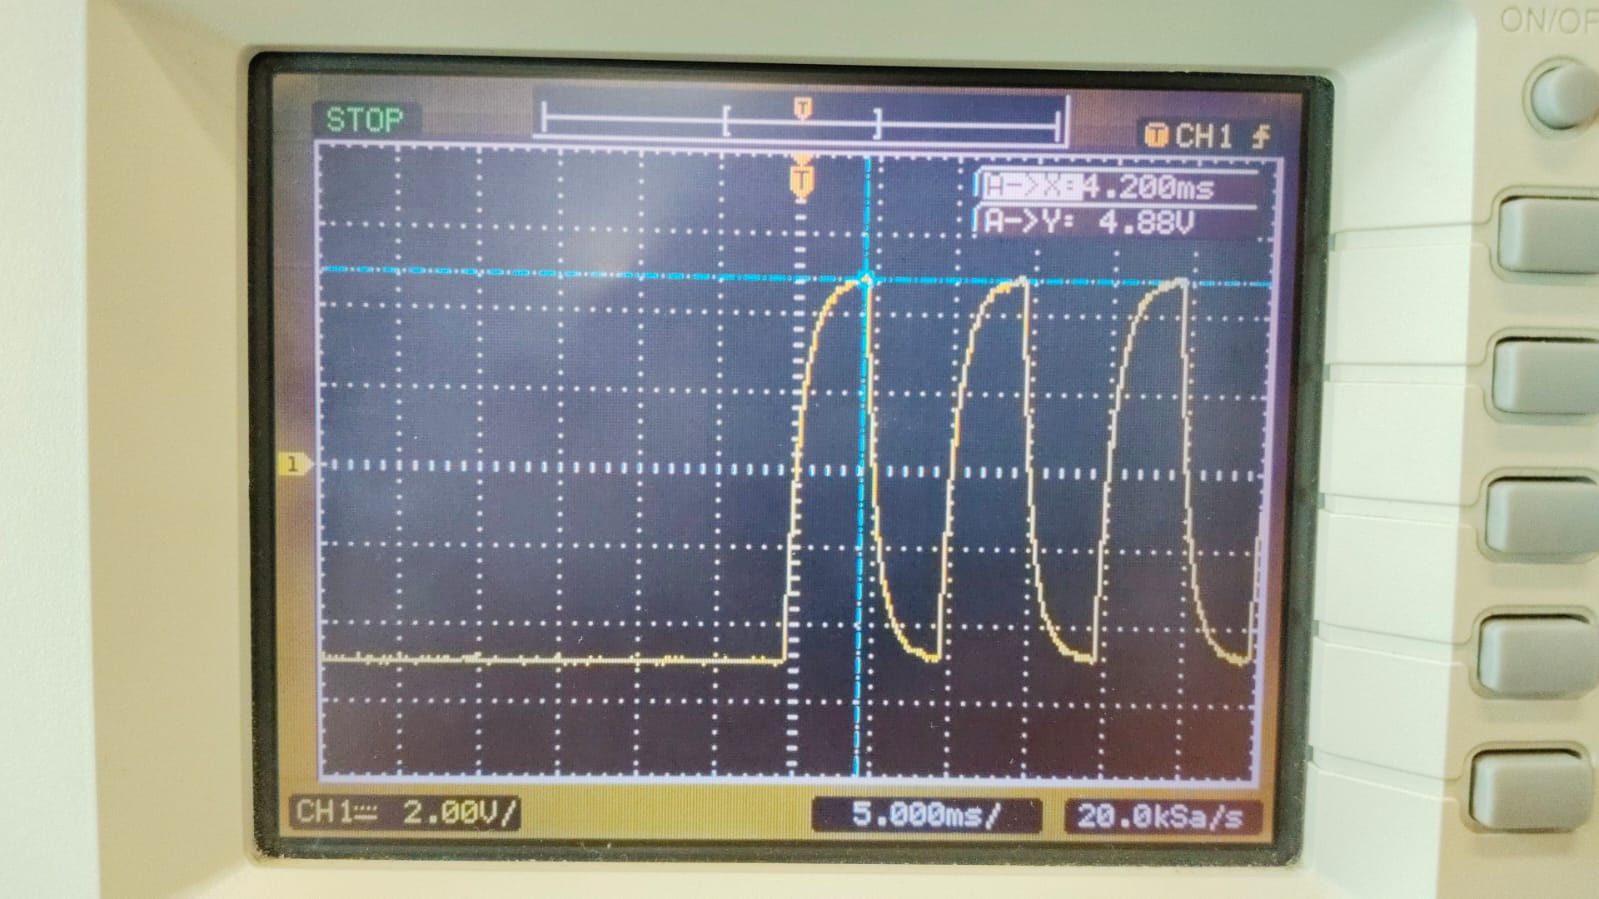
\includegraphics[width=\textwidth]{figs/rc<t_tr.jpeg}
    \caption{Transient Response for the first 5 cycles : \( RC \ll T \)}
\end{figure}

\section*{Comparison of CRO Measurements with Hand Calculations}
To verify the accuracy of the measurements from the oscilloscope, hand calculations were performed for the expected charging/discharging behavior of the capacitor. The voltage values and time periods observed on the oscilloscope were compared with these theoretical predictions.

\begin{itemize}
    \item For Case 1, the measured time constants closely matched the theoretical values calculated based on the square wave frequency.
    \item For Case 2, the oscilloscope readings confirmed the low-pass filtering effect, and the steady-state output had minimal ripple.
    \item For Case 3, the output closely tracked the input, confirming that the capacitor was charging and discharging rapidly enough to follow the square wave input.
\end{itemize}

\section*{Conclusion}
The behavior of the RC circuit in response to a square wave input was analyzed for three different conditions of the time constant. The results were consistent but with some errors because of the resistors and capacitors not being correctly calibrated, and the oscilloscope measurements confirmed the accuracy of the hand calculations. 

\end{document}
